\documentclass{ximera}

\graphicspath{
{./}
{../whatIsXimera/}
{../settingUpTheRepository/}
{../sageMathCloud/}
}


\title{LTI support}
\outcome{Use LTI to pass grades to an LMS.}
\begin{document}
\begin{abstract}
Ximera can use LTI to pass grades to an LMS.
\end{abstract}
\maketitle

\section{Key and secret}

To deploy Ximera activities as an assignment in an LMS using LTI you
must have a ``key'' and a ``secret'' given to you by Ximera. This key
and secret combination can be used by any user to set up homework on
an LMS. If we didn't have key's and secrets, students could (in
theory) submit grades directly to the LMS. The key-secret combo simply
validates to the LMS that the work came from some Ximera activity.

First recall your key using the command:

\begin{verbatim}
gpg --list-keys
\end{verbatim}


To get an authentic key-secret combination, do this:

\begin{verbatim}
xake -k YOUR-GPG-KEY lti NAME
\end{verbatim}
for example it might look like:
\begin{verbatim}
xake -k LKJ987LKJLKJ55JGHJKG77JKJ9898KLLKJLKJ99K lti mathassignments
\end{verbatim}
Then \verb|xake| will return:
\begin{verbatim}
SD4GSdFG4sDGF45ADfdgfsgf4542545sdfd245_j354 lti mathassignments
LTI key: mathassignments
 secret: 9KJ_83klkdiKLk956nK9_klsdKll-KJsdop998_kld7        
\end{verbatim}

will give you a key and secret. Note, repeating the same process will
always give you the same key-secret combination. You may share your
key-secret combination between faculty teaching any course with Ximera
activities.

\section{Canvas}

For each assignment there are two steps: Making an external tool and connecting an assignment to the external tool.

\subsection{Making and external tool}

For each assignment you want to add, start by going to Settings $\to$  Apps $\to$ View App Configurations

\begin{image}
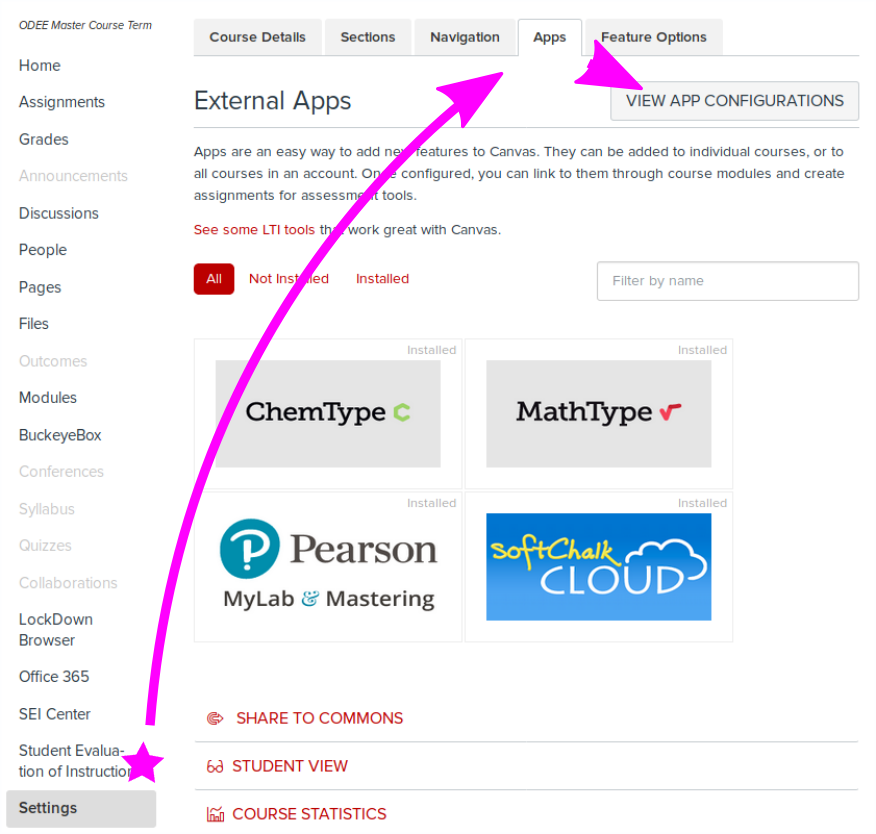
\includegraphics{canvas1.png}
\end{image}
Click on View App Configurations, 

\begin{image}
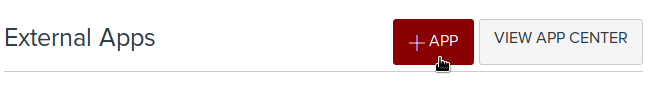
\includegraphics{canvas2.png}
\end{image}
and then click $+$APP
\begin{image}
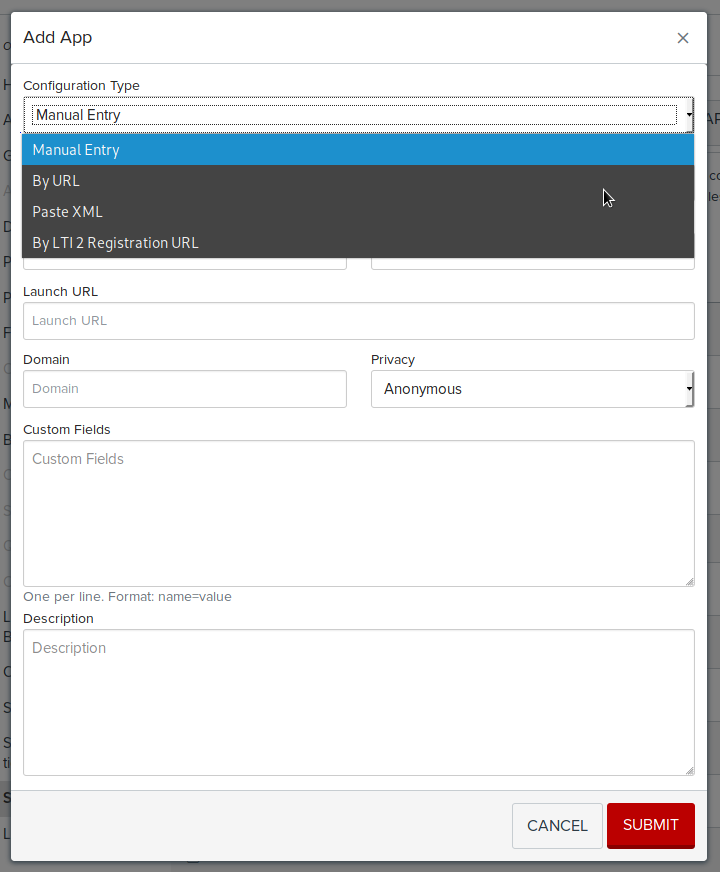
\includegraphics{canvas3.png}
\end{image}
and as we see above, choose configuration type ``By URL.''
Name it whatever you want to call it so you can find it again.
The key and secret are the ones from 'xake lti NAME' a minute ago.
The Config URL is ``https://ximera.osu.edu/COURSE/PATH/TO/EXERCISELIST/lti.xml.'' For example:
\begin{image}
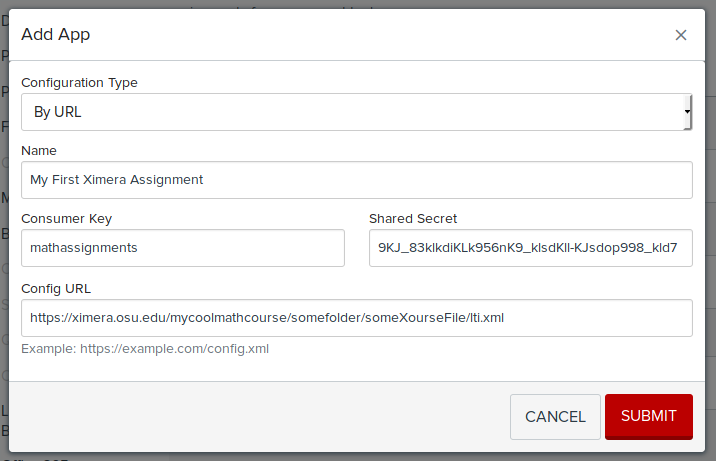
\includegraphics{canvas4.png}
\end{image}
This makes it so that you can connect an assignment to this external tool.

\subsection{Connecting an  assignment to the external tool}

Click on ``Assignments'' then $+$ASSIGNMENT. Name the assignment, assign points to the assignment, 
set the Submission Type to ``External Tool'' then find your assignment in the list:
\begin{image}
  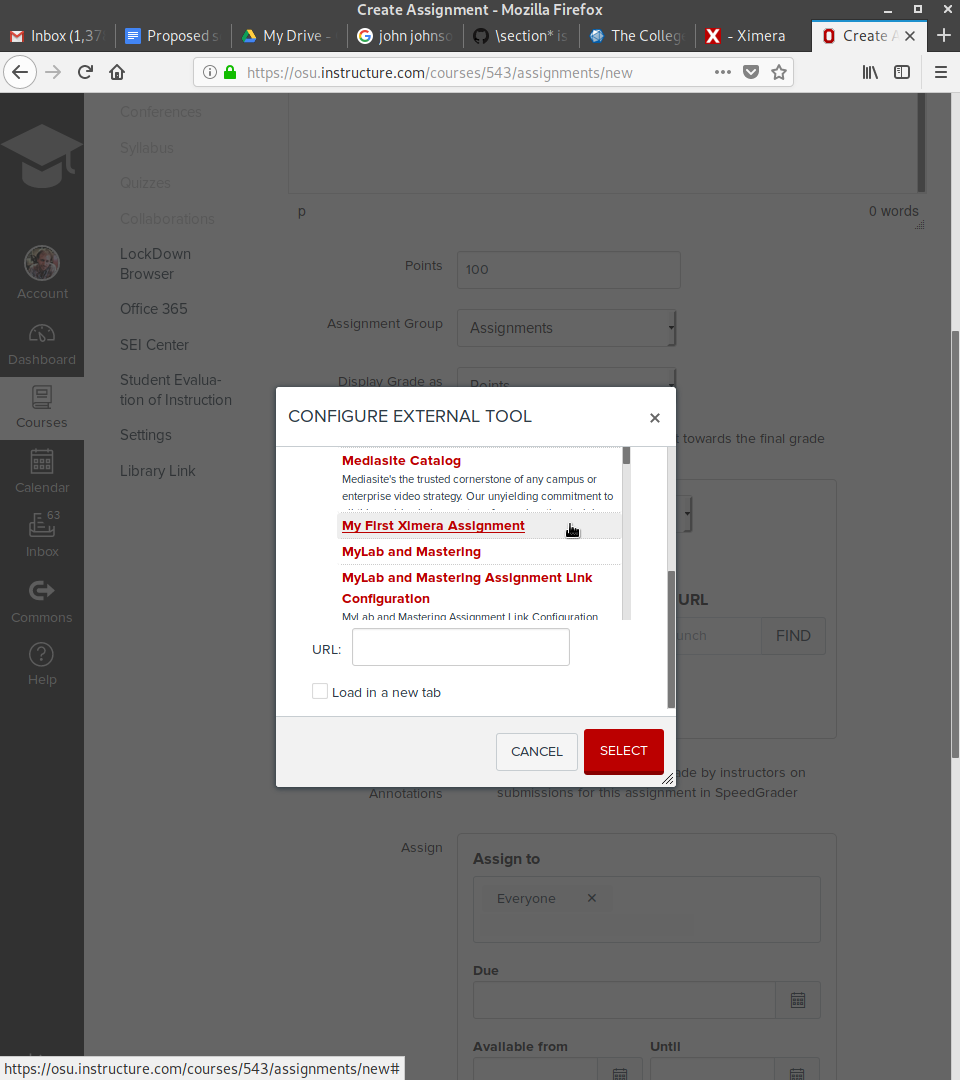
\includegraphics{canvas5.png}
\end{image}
The URL  for your assignment will be
\[
\texttt{https://ximera.osu.edu/COURSE/PATH/TO/EXERCISELIST/lti}
\]
\begin{warning}
Select Load Tool in New Window Tab, or else \textbf{we may not be able to record student data!}
\begin{image}
  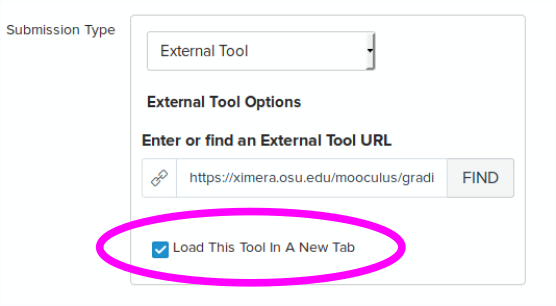
\includegraphics{canvas6.png}
\end{image}
\end{warning}
Finally, \textbf{remember to Save and Publish.}


%%         Save and Publish
        
%%         Click on the link to check it out.
        
%% As an instructor logged into ximera, click on your name/supervise to see what students are working on in real-time.  You
%%         can interact with the page and changes are visible to the student 

%% In Canvas:
%%         Settings > Student View to see site as a student
        
%% To see a student's work:
%%         Grades > Student Name > Their Assignment


\end{document}
